\documentclass[a4paper,12pt]{article}
\usepackage{fancyhdr}
\usepackage{graphicx}
\usepackage[export]{adjustbox}
\usepackage{caption}
\usepackage{float}
\usepackage{subcaption}

\graphicspath{ {./} }
\title{Latex cheatsheet}
\date{2021\\February}
\author{Frederik Lassen}
\pagestyle{fancy}
\fancyhf{}
\fancyfoot[R]{\thepage}
\renewcommand{\labelitemii}{$\star$}


\begin{document}
\maketitle
\thispagestyle{empty}
\clearpage
\pagenumbering{arabic}

\tableofcontents
\clearpage

\section{Introduction}
How to make danish letters
Æ Ø Å æ ø å
\section{Graphics}
\label{sec:graphics}
Let's find a picture of a cake
{
\begin{figure}[H]
	\centering
	\captionsetup{justification=centering}
	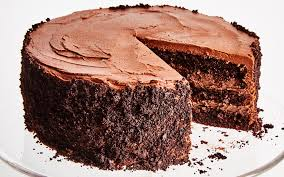
\includegraphics[scale=0.5]{cake}
	\caption{caption below, centered}
	\label{fig:cake1}
\end{figure}
}
Delicious cake. This text is not left alligned perfectly and i dont know why.
{
\begin{figure}[H]
	\centering
\begin{subfigure}{.5\textwidth}
	\centering
	\caption{caption above, left}
	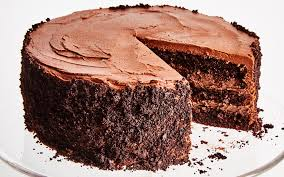
\includegraphics[width=.4\linewidth]{cake}
	\label{fig:cake2}
\end{subfigure}%
\begin{subfigure}{.5\textwidth}
	\centering
	\caption{caption above, right}
	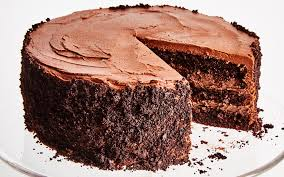
\includegraphics[width=.4\linewidth]{cake}
	\label{fig:cake3}
\end{subfigure}%
\caption{A figure with 2 subfigures}
\label{fig:double}
\end{figure}
}

\section{References}
Reference to first cake picture  ~\ref{fig:cake1} on page ~\pageref{fig:cake1} \\
Reference to second cake picture ~\ref{fig:cake2} on page ~\pageref{fig:cake2} in section ~\ref{sec:graphics} \\
Reference to third cake picture in subfigure ~\ref{fig:cake3} in  figure ~\ref{fig:double} on page ~\pageref{fig:cake3} in section ~\ref{sec:graphics}

\section{Sections}
Sections are by default numbered.
\section*{Non-numbered section}
\addcontentsline{toc}{section}{Non-numbered section}
But this one isn't
\section{Lists}
\begin{itemize}
\item this
\item is a
\item bullet point list
\end{itemize}
Break text
\begin{itemize}
\item this 
\item is a 
	\begin{itemize}
		\item stars!
		\item more stars!
	\end{itemize}
\item bullet point list
\end{itemize}
Break text
\begin{enumerate}
\item now they
\item have numbers
	\begin{enumerate}
	\item now they have letters
		\begin{enumerate}
		\item now they're roman
			\begin{enumerate}
			\item Capital letters!
			\end{enumerate}
		\end{enumerate}
	\end{enumerate}
\end{enumerate}

\section{Tables}


\end{document}